\documentclass[tikz,border=2pt,11pt]{standalone}
\usetikzlibrary{arrows.meta}
\usetikzlibrary{fit}
\usetikzlibrary{decorations.pathreplacing}
\usetikzlibrary{backgrounds}
\usetikzlibrary{calc}
\usetikzlibrary{patterns}
\usetikzlibrary{positioning}
\usepackage{amsmath}
\usepackage{amssymb}
\usepackage{tikz}
\usepackage{xcolor}
\DeclareMathOperator{\Env}{Env}
\DeclareMathOperator{\rank}{rank}
\DeclareMathOperator{\mult}{mult}
\DeclareMathOperator{\Span}{span}
\DeclareMathOperator{\codim}{codim}
\DeclareMathOperator{\Spec}{Spec}
\DeclareMathOperator{\Sing}{Sing}
\DeclareMathOperator{\supp}{supp}
\DeclareMathOperator{\tr}{tr}
\DeclareMathOperator{\Res}{Res}
\DeclareMathOperator{\lcm}{lcm}
\newcommand{\R}{\mathbb R}
\newcommand{\C}{\mathbb C}
\newcommand{\PP}{\mathbb P}
\newcommand{\E}{\mathbb E}
\newcommand{\Prob}{\mathbb P}
\begin{document}
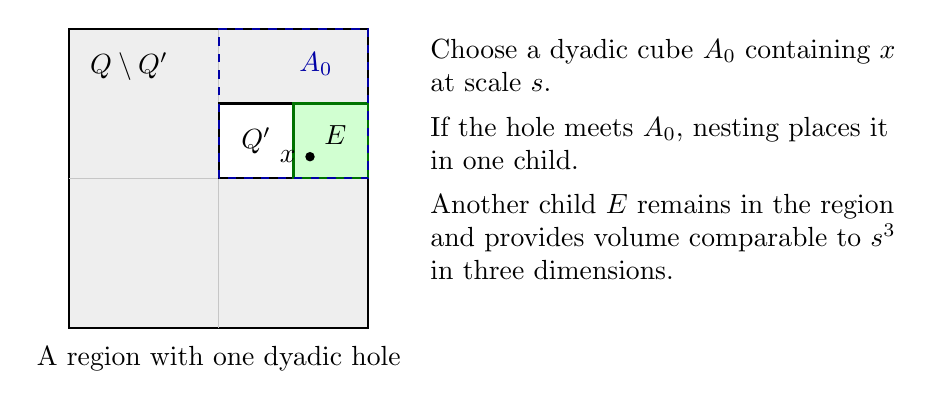
\begin{tikzpicture}[scale=0.95]
 \fill[gray!13] (0,0) rectangle (4,4);
 \draw[thick] (0,0) rectangle (4,4);
 \draw[gray!45] (2,0)--(2,4) (0,2)--(4,2);
 \fill[white] (2,2) rectangle (3,3);
 \draw[thick] (2,2) rectangle (3,3);
 \fill[green!18] (3,2) rectangle (4,3);
 \draw[green!45!black,thick] (3,2) rectangle (4,3);
 \draw[blue!65!black,dashed,thick] (2,2) rectangle (4,4);
 \fill (3.22,2.29) circle (1.8pt);
 \node[anchor=east] at (3.16,2.29) {$x$};
 \node at (2.5,2.5) {$Q'$};
 \node at (3.56,2.58) {$E$};
 \node[blue!65!black] at (3.3,3.53) {$A_0$};
 \node at (0.8,3.5) {$Q\setminus Q'$};
 \node[anchor=north] at (2,-0.12) {A region with one dyadic hole};
 \node[align=left,anchor=west,text width=6.0cm] at (4.7,2.25)
 {Choose a dyadic cube $A_0$ containing $x$ at scale $s$.\\[4pt]
  If the hole meets $A_0$, nesting places it in one child.\\[4pt]
  Another child $E$ remains in the region and provides volume
  comparable to $s^3$ in three dimensions.};
\end{tikzpicture}
\end{document}
